\documentclass[arhiv]{izpit}

\begin{document}

%==========================================================================
%               Sem vpisi podatke o izpitu
%==========================================================================
\FRACTIONSIMPLIFY{31}{1}{\skupnotock}{\nepomembno}%Sem vpiši (v polje trenutno {60}) skupno število točk, da paket naračuna kriterij ocenjevanj
\izpit[ucilnica = RAZRED, naloge = 6]%ucilnica RAZRED, lahko se sedezni red, ime in priimek, maturitetni
{Matematika - Geometrija}{22. 9. 2023}{Čas pisanja je 45 minut.\\ Možno je doseči $\skupnotock$ točk.\\ Veliko uspeha!}
%==========================================================================
%               Nepomembno - Preskoči
%==========================================================================
\MAX{0.1}{0}{\tempepsilon}%shranimo epsilon... ne gre trik z ulomkom zato max
\MULTIPLY{\skupnotock}{0.9}{\odlicno}
\MULTIPLY{\skupnotock}{0.76}{\pravdobro}
\MULTIPLY{\skupnotock}{0.63}{\dobro}
\MULTIPLY{\skupnotock}{0.5}{\zadostno}
\ADD{\dobro}{\tempepsilon}{\dobroplus}
\ADD{\pravdobro}{\tempepsilon}{\pravdobroplus}
\ADD{\odlicno}{\tempepsilon}{\odlicnoplus}
\ROUND[0]{\dobroplus}{\dobroplus}
\ROUND[0]{\pravdobroplus}{\pravdobroplus}
\ROUND[0]{\odlicnoplus}{\odlicnoplus}
\ROUND[0]{\zadostno}{\zadostno}
\ROUND[0]{\dobro}{\dobro}
\ROUND[0]{\pravdobro}{\pravdobro}
\ROUND[0]{\odlicno}{\odlicno}\begin{small}
 \PlaceText{100mm}{33mm}{\begin{tabular}{ll}
    \multicolumn{2}{c}{\textbf{Kriterij ocenjevanja}} \\[0.5ex]
    Ocena & Tocke \\ \hline
    zadostno & $\zadostno - \dobro$ \\
    dobro & $\dobroplus - \pravdobro$ \\
    prav dobro & $\pravdobroplus - \odlicno$ \\
    odlicno & $\odlicnoplus$--
  \end{tabular}}\end{small}
 \ifthenelse{\boolean{@maturitetni}}{\newpage}%TO JE ZELO GRDA KODA a ker ne gre kriterij v class ni druge moznosti
%==========================================================================
%               Sem vpisi naloge
%   za dodatek koordinatnega sistema daj pod navodila naloge \dodatek{\[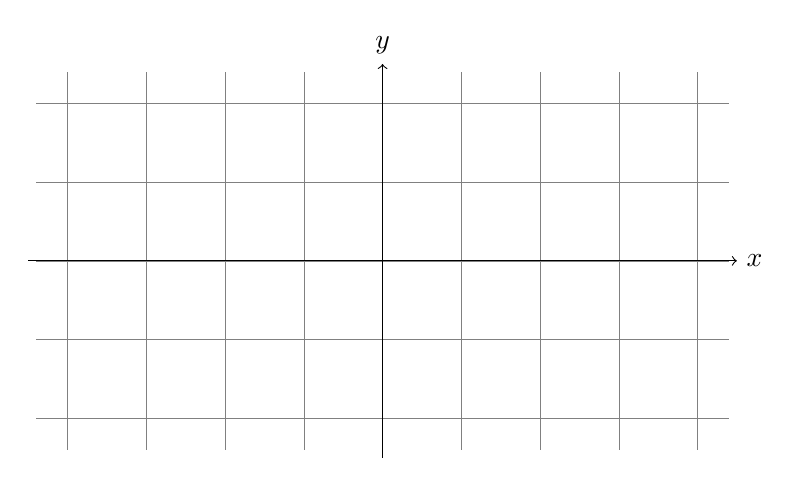
\begin{tikzpicture}
        \draw[help lines,step=1cm] (-4.4,-2.4) grid (4.4,2.4);
        \draw[->] (-4.5,0) -- (4.5,0) node[right] {$x$};
        \draw[->] (0,-2.5) -- (0,2.5) node[above] {$y$};
\end{tikzpicture}\]}
%   oz. za kompleksno ravnino \dodatek\[\begin{tikzpicture}
        \draw[help lines,step=1cm] (-4.4,-2.4) grid (4.4,2.4);
        \draw[->] (-4.5,0) -- (4.5,0) node[right] {$Re$};
        \draw[->] (0,-2.5) -- (0,2.5) node[above] {$Im$};
\end{tikzpicture}\]
%==========================================================================

\naloga[\tocke{8}]
  \podnaloga[4]
  Načrtaj paralelogram s podatki $\alpha=60^\circ$, $a=6cm$ in $e=8cm$. Bolje naloge s podanim a+c...
  \prostor[1]
  \podnaloga[4]
  Načrtaj trikotnik s podatki $\gamma =30^\circ$, $c=5cm$ in $t_c =4cm$. Naj bo teziscnica in kot npr. 90 stopinj
  \prostor[1]


  
\naloga[\tocke{8}]
  \podnaloga[4]
  V trapezu $ABCD$ sta kota $\angle ADC$ in $\angle ACB$ enaka. Izračunaj dolžino diagonale $e$, če sta osnovnici dolgi $a=9cm$ in $c=4cm$.
  \prostor[2]
  \podnaloga[4]
  Število diagonal v nekem pravilnem večkotniku je za 25 večje od števila stranic. Izračunaj, koliko meri notranji kot tega večkotnika.
  \prostor[1]


\naloga[\tocke{8}]
  \podnaloga[4]
  V pravokotnem trikotniku merita pravokotni projekciji katet na hipotenuzo $18cm$ in $32cm$. Izračunaj, koliko merijo stranice tega trikotnika
  \prostor[1]
  \podnaloga[4]
  Trigonometrija
  \prostor[1]





\end{document}